About the scheduler and Ready Threads Queue

\par
\par
\par
\hypertarget{scheduler_sched_quantum}{}\subsection{Quantum}\label{scheduler_sched_quantum}
The period of time for which a thread is allowed to execute in a preemptive multi-\/threading system is generally called the time slice, or {\ttfamily quantum}. The scheduler is run once every quantum to choose the next thread for execution. If the quantum is too short then the scheduler overhead may become high.

An interrupt is used to allow the kernel to switch between threads when their quantum expires, effectively allowing the processor's time to be shared between a number of threads, giving the illusion that it is dealing with these threads concurrently.\hypertarget{scheduler_sched_thdL}{}\subsection{Threads List}\label{scheduler_sched_thdL}
Each thread structure \hyperlink{structesThd}{es\-Thd} contains Thread List structure \hyperlink{structesThd_1_1thdL}{es\-Thd\-::thd\-L}. All threads of the same priority are linked together via {\itshape next} and {\itshape prev} members in \hyperlink{structesThd_1_1thdL}{es\-Thd\-::thd\-L} structure. The first member of the structure is pointer {\itshape q} which points back to the Threads Queue structure (\hyperlink{structesThdQ}{es\-Thd\-Q}) which contains the threads.

The list is organized as {\bfseries circular doubly linked list}, which means that {\itshape tail} and {\itshape head} nodes are linked together just like every other node in the list. This provides easy and efficient traversal of the list.


\begin{DoxyImage}
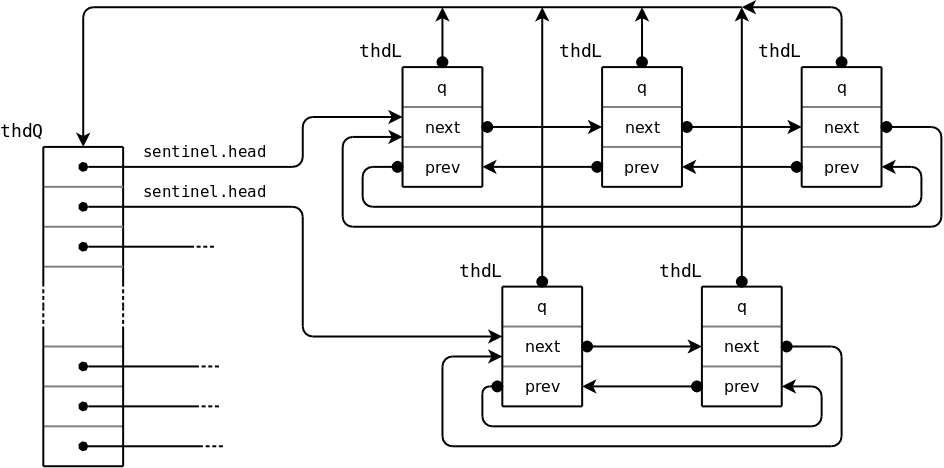
\includegraphics[width=12cm]{thdL.png}
\caption{Detailed view of Threads List (sentinel.next pointers not shown)}
\end{DoxyImage}


Each sentinel of a list has two pointers, {\itshape head} and {\itshape next}. Pointer sentinel.\-head$\ast$ always points to the first entry of the list which is called head$\ast$. Every new thread is added at the {\itshape tail} of the list which is essentialy just after the node {\itshape head}. When a first thread is added to the list the pointer sentinel.\-next$\ast$ points to the thread, too. When the list is rotated using function \hyperlink{group__kern__intf_gae365b14292f1496a90d876baec84fb4e}{es\-Thd\-Q\-Fetch\-Rotate\-I()} the pointer {\itshape sentinel.\-next} is advanced forward and points to the next thread in list.


\begin{DoxyImage}
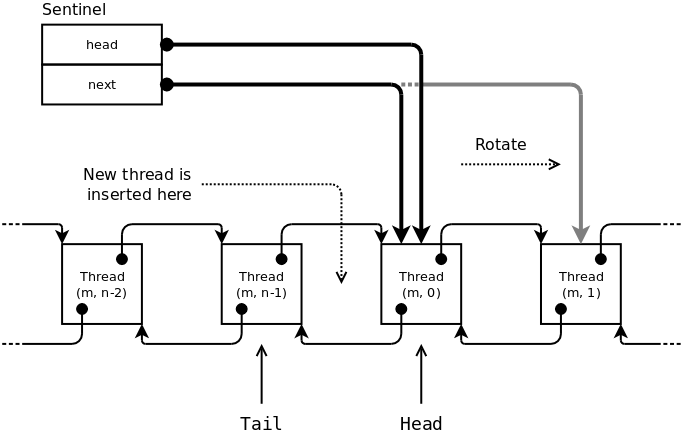
\includegraphics[width=12cm]{thdL-rotate.png}
\caption{Detailed view of the sentinel and linked list}
\end{DoxyImage}
\hypertarget{scheduler_sched_thdQ}{}\subsection{Threads Queue}\label{scheduler_sched_thdQ}
Based on the number of configured priority levels (see \hyperlink{group__template__kern__cfg_ga56bd89fe76f7fe22f3d8805bc3c68892}{C\-F\-G\-\_\-\-S\-C\-H\-E\-D\-\_\-\-P\-R\-I\-O\-\_\-\-L\-V\-L}) and on the number of data register bits (see \hyperlink{group__template__cpu__intf_gac4d9e19c50315dec7721d4bc4d6b0605}{P\-O\-R\-T\-\_\-\-D\-A\-T\-A\-\_\-\-W\-I\-D\-T\-H\-\_\-\-V\-A\-L}) of the used C\-P\-U, two configurations are possible\-:
\begin{DoxyItemize}
\item Simple Ready Threads Queue
\item Complex Ready Threads Queue
\end{DoxyItemize}

Simple Ready Threads Queue configuration is used when the number of configured priority levels is lower or equal to the number of bits in general purpose data register. For example if application is using 9 priority levels on 32-\/bit C\-P\-U than simple Ready Threads Queue configuration is used. In contrast, when using 9 priority levels on an 8-\/bit C\-P\-U than the kernel is forced to use the Complex Ready Threads Queue configuration since 8-\/bit register cannot carry 9 bits of data.\hypertarget{scheduler_sched_rdyThdQ_simple}{}\subsubsection{Simple Ready Threads Queue}\label{scheduler_sched_rdyThdQ_simple}
Each bit in {\ttfamily bit\mbox{[}0\mbox{]}} variable represents one priority level. The number of bits used in this variable depends on \hyperlink{group__template__kern__cfg_ga56bd89fe76f7fe22f3d8805bc3c68892}{C\-F\-G\-\_\-\-S\-C\-H\-E\-D\-\_\-\-P\-R\-I\-O\-\_\-\-L\-V\-L} value. If a bit at {\ttfamily Nth} position is set then there is a thread inserted in Thread List at {\ttfamily Nth} priority level.

\par

\begin{DoxyImage}
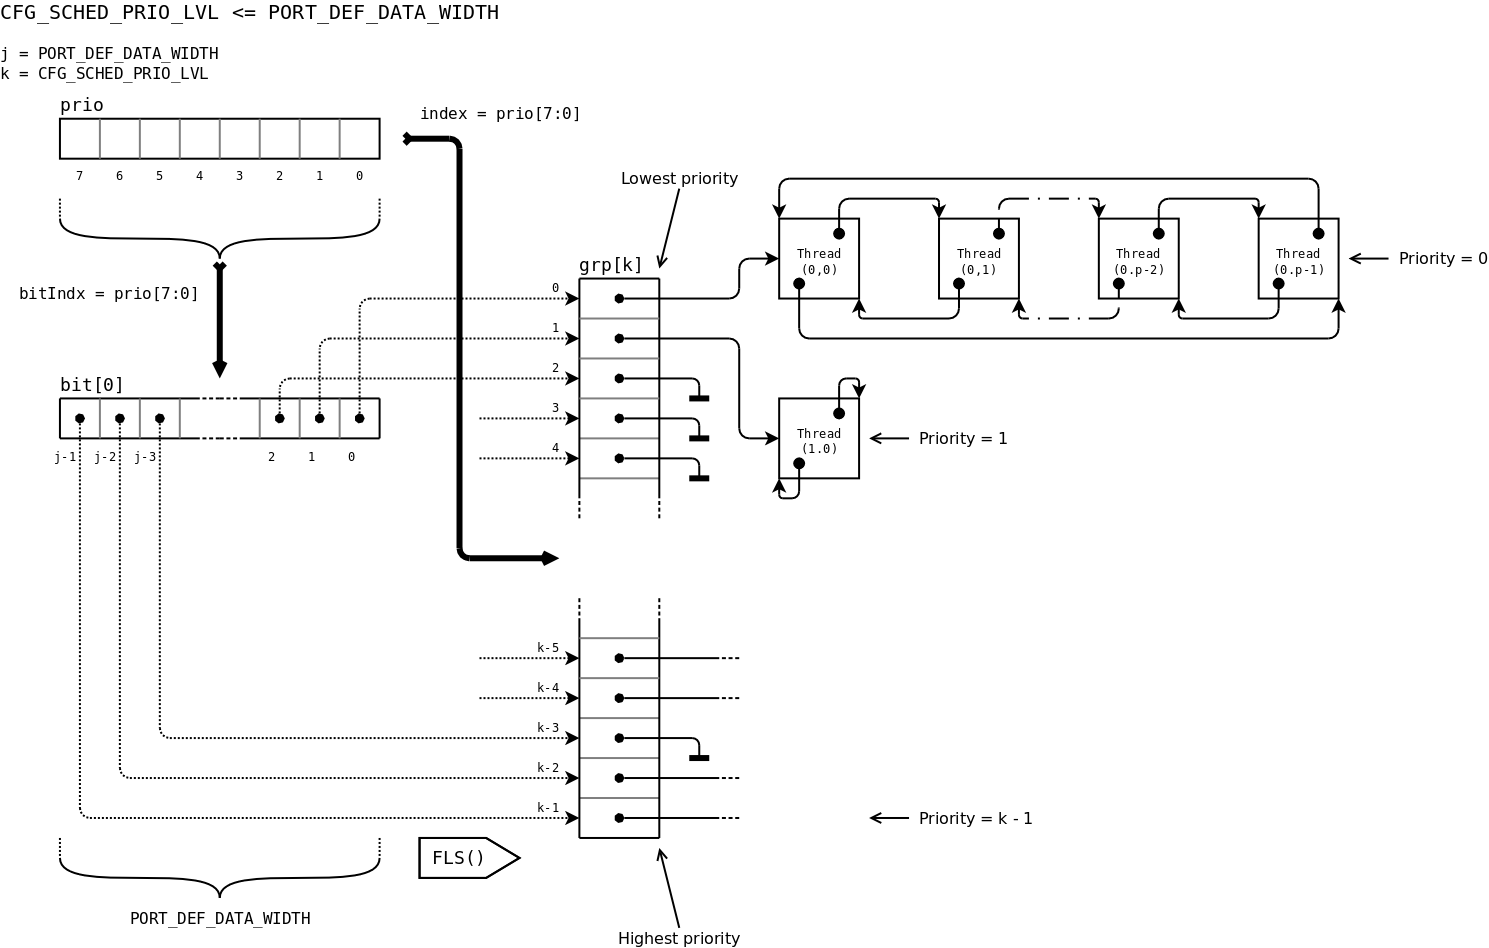
\includegraphics[width=15cm]{thdQ-simple.png}
\caption{Ready Threads Queue -\/ low number of priority levels}
\end{DoxyImage}


\begin{DoxyParagraph}{Inserting a thread}
The process of a thread insertion into a thread queue can be described using the following pseudo-\/code\-: 
\begin{DoxyCode}
\textcolor{keyword}{function} insert(thread)
    priority := thread.priority                             \textcolor{preprocessor}{# Get the priority of the thread}
\textcolor{preprocessor}{}    
    \textcolor{keywordflow}{if} (grp[priority].head == NULL)                         # If \textcolor{keyword}{this} priority level has a list
        grp[priority].head := thread                        # Create a list with \textcolor{keyword}{this} thread as head
        grp[priority].next := thread
        bitIndx := 2^priority                               # bitIndx equals to 2 raised to the power of 
      priority
        bit[0]  := bit[0] or bitIndx                        # Set the calculated bit in Bit Map
    \textcolor{keywordflow}{else}
        listInsertAtTail(grp[priority].head, thread)        \textcolor{preprocessor}{# Add thread at tail of existing list}
\textcolor{preprocessor}{}    end \textcolor{keywordflow}{if}
end \textcolor{keyword}{function}
\end{DoxyCode}

\end{DoxyParagraph}
\begin{DoxyParagraph}{Removing a thread}
The process of a thread removal can be described with the following pseudo-\/code\-: 
\begin{DoxyCode}
\textcolor{keyword}{function} \textcolor{keyword}{remove}(thread)
    priority := thread.priority                             # Get the priority of the thread
    
    if (listIsEntryLast(thread))                            # In \textcolor{keywordflow}{case} we are removing the last entry
        grp[priority].head := NULL                          # List is deleted
        bitIndx := 2^priority                               # bitIndx equals to 2 raised to the power of 
      priority
        bit[0]  := bit[0] and not bitIndx                   # Clear the calculated bit in Bit Map
    \textcolor{keywordflow}{else}
        listRemove(thread)                                  # Remove the thread from list
    end \textcolor{keywordflow}{if}
end \textcolor{keyword}{function}
\end{DoxyCode}

\end{DoxyParagraph}
\begin{DoxyParagraph}{Fetching the highest priority thread}
The process of fetching the highest priority thread is inverse function of {\ttfamily 2$^\wedge$priority} which was used in {\ttfamily insert()} function\-: 
\begin{DoxyCode}
\textcolor{keyword}{function} fetch()
    priority := log2(bit[0])                                \textcolor{preprocessor}{# Find Last Set bit position in bit[0]}
\textcolor{preprocessor}{}
    \textcolor{keywordflow}{return} grp[priority]
end \textcolor{keyword}{function}
\end{DoxyCode}

\end{DoxyParagraph}
\begin{DoxyParagraph}{Rotating the threads queue}
The process can be described with the following algorithm\-: 
\begin{DoxyCode}
\textcolor{keyword}{function} rotate()
    priority := log2(bit[0])                                \textcolor{preprocessor}{# Find Last Set bit position in bit[0]}
\textcolor{preprocessor}{}
    grp[priority].next := grp[priority].next.next
    
    \textcolor{keywordflow}{return} grp[priority].next
end \textcolor{keyword}{function}
\end{DoxyCode}
 
\end{DoxyParagraph}
\hypertarget{scheduler_sched_rdyThdQ_complex}{}\subsubsection{Complex Ready Threads Queue}\label{scheduler_sched_rdyThdQ_complex}

\begin{DoxyImage}
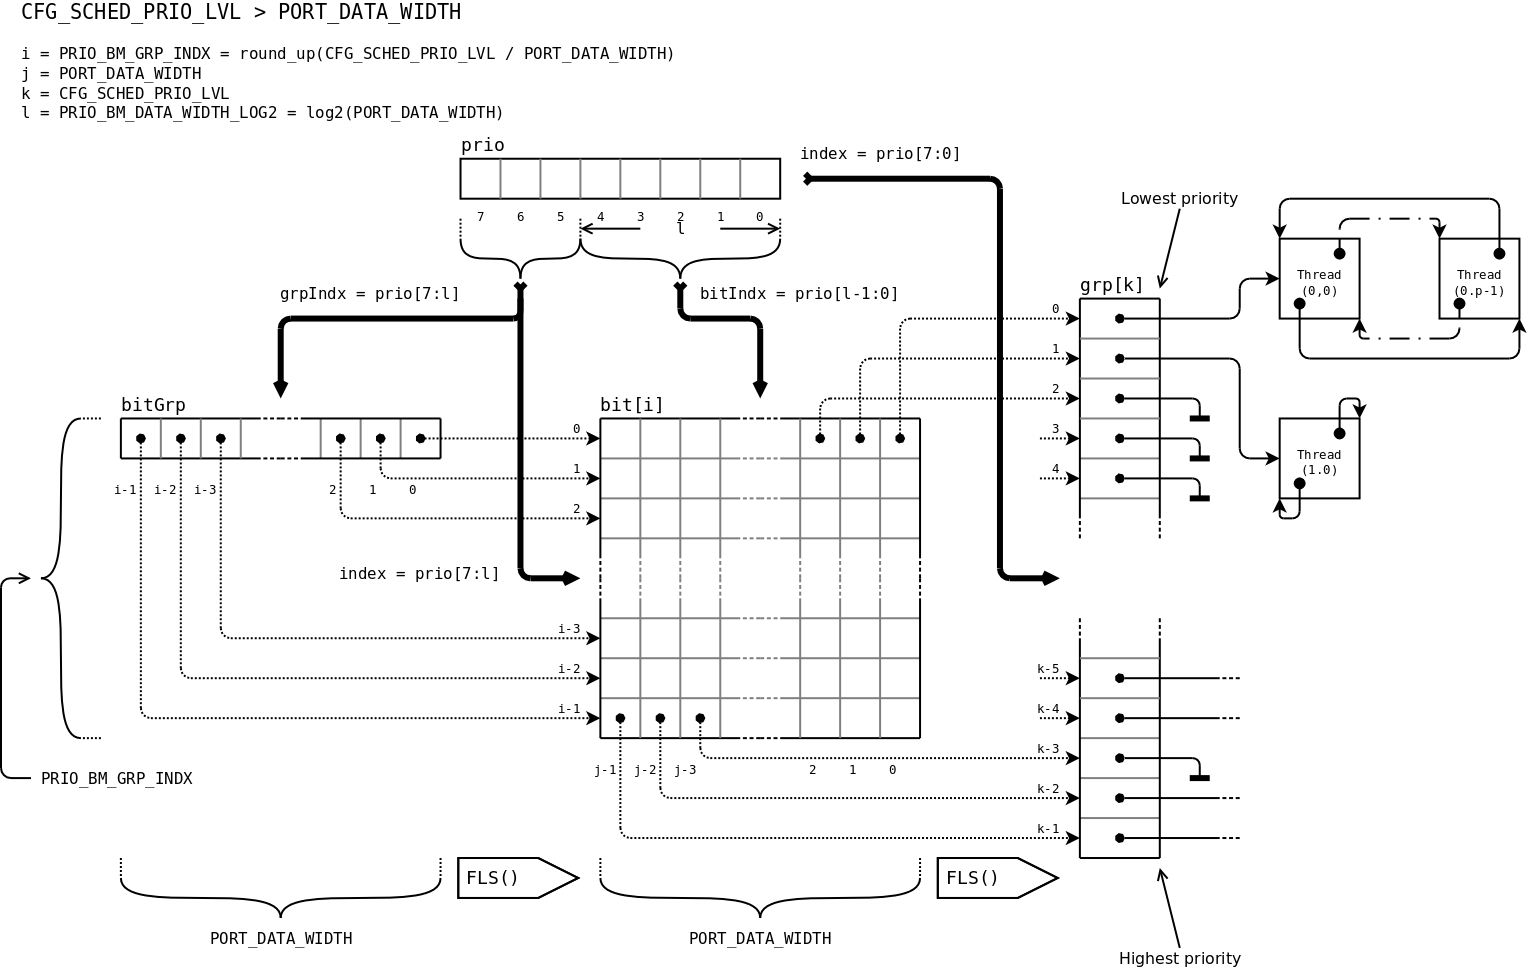
\includegraphics[width=17cm]{thdQ-complex.png}
\caption{Ready Threads Queue -\/ high number of priority levels}
\end{DoxyImage}
\hypertarget{scheduler_sched_rdyThdQ}{}\subsection{Ready Threads Queue}\label{scheduler_sched_rdyThdQ}
Ready Threads Queue holds threads that are ready for execution. 